\chapter{Additional Background}
\section{Ontology}
\subsection{Terminology, Taxonomy and Ontology}
Terminology is a system or collection of words. The system is managed to make content more consistent and standardized. Terminology helps improve readability, translation, and brand perception \cite{TaxonomyVSTerminology}.

A taxonomy is a way to classify words into hierarchical groups. The biggest use of a taxonomy is for search.
A taxonomy defines groups of words. It can be multi-layered or flat \cite{TaxonomyVSTerminology}.

An ontology describes a concept both by its position in a hierarchy and its relationships to other concepts. The richness of the relationships described in an ontology is what makes more powerful for modeling complex systems \cite{OntologyHasRicherRelationshipThanTaxonomy}.

In computer-science Taxonomy has been adopted to name trees of generalization-specialization relation. In ontologies can be build over any kind of relationships, including generalization-specialization and many other.
Taxonomies and ontologies usually concern terms but they are not limited to such. In terms of graph theory, taxonomies are trees, and ontologies are graphs or hyper-graphs, where edges are build from many different relations. Those relation could have any properties according to set theory \cite{taxonomiesRtreesOntologiesRgraphs}.

\subsection{Ontology versus Database}

For those who are familiar with database, ontology axioms are like DB schema.
In database, schema describes structure of and constraints on data.
Ontology facts are like DB data, they are consistent with schema constraints \cite{OntologyLanguageTool2}.
For differences, see table \ref{table:ontology_vs_database}. 
The given examples are expressed with Description Logic, see Section \ref{sec:DL} for more details.

\begin{longtable}[ht]{| p{65mm} | p{65mm} |} 
\hline
\rowcolor{orange} Database & Ontology\\
\hline
\rowcolor{green} Closed word assumption (CWA) & Open world assumption (OWA)\\ 
Missing information treated as false & Missing information treated as unknown\\
\hline
\rowcolor{lightgray} \multicolumn{2}{|c|}{For example, we have the following facts/data:}\\
\rowcolor{lightgray} \multicolumn{2}{|c|}{HarryPotter hasFriend RonWeasley}\\
\rowcolor{lightgray} \multicolumn{2}{|c|}{HarryPotter hasFriend HermioneGranger}\\
\hline
\multicolumn{2}{|c|}{Query: Is Draco Malfoy a friend of HarryPotter?}\\
\hline
DB: No & Ontology: Don’t Know (didn’t say Draco was not Harry’s friend)\\
\hline
\rowcolor{green} Unique name assumption (UNA) & No UNA \\ 
Each individual has a single unique name & Individuals may have more than one name\\
\hline
\multicolumn{2}{|c|}{How many friends does Harry Potter have?}\\
\hline
DB: 2 & Ontology: at least 1 (Ron and Hermione may be 2 names for same person)\\
\hline
\rowcolor{green} Schema behaves as constraints on structure of data & Ontology axioms behave like implications (inference rules) \\ 
\hline
\rowcolor{lightgray} \multicolumn{2}{|c|}{For example, if we try to add new facts/data:}\\
\rowcolor{lightgray} \multicolumn{2}{|c|}{Dumbledore: Wizard}\\
\rowcolor{lightgray} \multicolumn{2}{|c|}{Fawkes: Phoenix}\\
\rowcolor{lightgray} \multicolumn{2}{|c|}{Fawkes isPetOf Dumbledore}\\
\rowcolor{lightgray} \multicolumn{2}{|c|}{$\exists hasPet.\top\subseteq Human$}\\
\rowcolor{lightgray} \multicolumn{2}{|c|}{$Phoenix\subseteq\forall isPetOf.Wizard$}\\
\hline
\rowcolor{gray} \multicolumn{2}{|l|}{Symbols}\\
\multicolumn{2}{|l|}{$\top$ \cite{top} tautology, top, Thing, most general concept}\\
\multicolumn{2}{|l|}{$\exists$ there exists at least one}\\
\multicolumn{2}{|l|}{$\subseteq$ is subset of}\\
\multicolumn{2}{|l|}{$\forall$ for all}\\
\hline
Update rejected: constraint violation. Domain of hasPet is Human; Dumbledore is not Human (CWA). &
Infer that Dumbledore is Human (domain restriction)\\ 
\hline
\rowcolor{green} \multicolumn{2}{|c|}{Query Answering Mechanism}\\
\hline
Schema plays no role & Ontology axioms play a powerful and crucial role\\
Data must explicitly satisfy schema constraints & Answer may include implicitly derived facts. Can answer conceptual as well as extensional queries, e.g., Can a Muggle have a Phoenix for a pet?\\ 
Query answering amounts to model checking, i.e., a “\textbf{look-up}” against the data & Query answering amounts to theorem proving, i.e., \textbf{logical entailment}\\ 
\textbf{Can be very efficiently implemented.} Worst case complexity is low (logspace) w.r.t. size of data. & \textbf{May have very high worst case complexity}, e.g., for OWL, NP-hard w.r.t. size of data
(upper bound is an open problem). Implementations may still behave well in typical cases.\\ 
\hline
\caption{Ontology versus Database}
\label{table:ontology_vs_database}
\end{longtable}

\subsection{Description Logic}
\label{sec:DL}

RDFS, and OWL support a family of knowledge representation languages called description logics (DL) \cite{DLExample}. A description logic can model concepts, roles and individuals, and their relationships. The common notations used in DL can be find in Table \ref{table:DL_notation}. Different DLs often with "strange names". see Table \ref{table:DL_naming_convention}
for more details, and Table \ref{table:DL_ontology_language} shows which DL is supported in which ontology language.

\begin{longtable}[h]{ p{10mm} p{60mm} p{15mm} p{45mm}}
\caption{Description Logic Notation}
\label{table:DL_notation}\\
\hline
\hline
Symbol & Description & Example & Read\\
\hline
$\top$ & tautology is a special concept with every individual as an instance, abbreviation for $A \sqcup \neg A$ for any concept A & $\top$ & top\\
\hline
$\bot$ & empty concept, contradiction, abbreviation for $A \sqcap \neg A$ for any concept A & $\bot$ & bottom\\
\hline
$\sqcap$ & intersection or conjunction of concepts & $ C \sqcap D $ & C and D\\
\hline
$\sqcup$ & union or disjunction of concepts	& $ C \sqcup D $ & C or D\\
\hline
$\neg$ & negation or complement of concepts	& $\neg C$ & not C\\
\hline
$\forall$ & universal restriction & $\forall R.C$ & all R-successors are in C\\
\hline
$\exists$ & existential restriction	& $\exists R.C$ & an R-successor exists in C\\
\hline
$\sqsubseteq$ & Concept inclusion, subclass relationship. & $ C \sqsubseteq D $ & all C are D\\
\hline
$ \equiv $ & Concept equivalence & $ C \equiv D $ &	C is equivalent to D\\
\hline
$\dot{=}$ & Concept definition & $ C \dot{=} D $ & C is defined to be equal to D\\
\hline
: &	Concept assertion & a:C & a is a C\\
\hline
: &	Role assertion & (a,b):R & a is R-related to b\\
\hline
\hline
\end{longtable}

\begin{longtable}[h]{ p{10mm} p{120mm} }
\caption{Description Logic Naming Convention: Meaning for Letters}
\label{table:DL_naming_convention}\\
\hline
Symbol & Constructs	and Example\\
\hline
$\mathcal{AL}$ & Attributive Language\\
& Atomic negation, concept intersection, universal restrictions, limited existential quantification\\
& $ copyrightHolder \equiv Organization \sqcup Person $\\
\hline
$\mathcal{C}$ & Complex concept negation\\
& Complex class expressions by combining mathematical operators such as subclass relationships, equivalence, conjunction, disjunction, negation, property restrictions, tautology, and contradiction\\
& $ cartoon \equiv animatedMovie \sqcap \neg (liveAction \sqcup computerAnimation) $\\
& Some DL languages have overlapping constructs, as, for example, union and full existential quantification can be expressed using negation, therefore $\mathcal{U}$ and $\mathcal{E}$ are never used together in DL names, and C is used instead.\\
\hline
$\mathcal{S}$ & An abbreviation for $\mathcal{ALC}$ with transitive roles\\
& $partOf \circ partOf \sqsubseteq partOf$\\
\hline
$\mathcal{E}$ &	Full existential qualification (existential restrictions that have fillers other than $\top$ )\\
& $ \exists hasDiscRelease.Blu-Ray $ \\
\hline
$\mathcal{F}$ &	Functional properties, a special case of uniqueness quantification.\\
& $ \top \sqsubseteq \leq 1$ officialWebsite$.\top $ \\
\hline
$\mathcal{U}$ &	Concept union\\
& $ broadcastChannel \equiv webcastChannel \sqcup televisionChannel $\\
\hline
$\mathcal{H}$ & Role hierarchy (subproperties: \texttt{rdfs:subPropertyOf})\\
& $ remakeOf \sqsubseteq basedOn $ \\
\hline
$\mathcal{R}$ & Limited complex role inclusion axioms; reflexivity and irreflexivity; role disjointness.\\
& $ supervisorOf \circ castMemberOf \sqsubseteq directorOf $ \\
\hline
$\mathcal{O}$ & Enumerated classes of object value restrictions (Nominals): \texttt{owl:oneOf}, \texttt{owl:hasValue}.\\
& $ AnimationStudios \equiv { DreamWorks, Walt Disney Animation Studios, Pixar }$\\
\hline
$\mathcal{I}$ &	Inverse properties.\\
& $ directedBy \approx directorOf^{-} $\\
\hline
$\mathcal{N}$ & Cardinality restrictions (\texttt{owl:cardinality}, \texttt{owl:maxCardinality}), a special case of counting quantification\\
& $ TVSeries \equiv \geq 2hasEpisode.\top $\\
\hline
$\mathcal{Q}$ & Qualified cardinality restrictions (available in OWL 2, cardinality restrictions that have fillers other than $\top$ ).\\
& $	Actor \sqsubseteq = 1hasBirthplace.Human $\\
\hline
$\mathcal{(D)}$ & Use of datatype properties, data values or data types.\\
& $\top\sqsubseteq\forall\geq 0zeroone.float$\\
& $\top\sqsubseteq\forall\leq 1zeroone.float$\\
& $\top\sqsubseteq\forall transparency.zeroone$\\
& $\exists transparency.\top \sqsubseteq Material$\\
\hline
\end{longtable}

In DL, a distinction is drawn between the so-called TBox (\textbf{terminological box}) and the ABox (\textbf{assertional box}). In general, the TBox contains sentences describing concept hierarchies (i.e., relations between concepts) while the ABox contains ground sentences stating where in the hierarchy individuals belong (i.e., relations between individuals and concepts). For example, the statement:

\blockquote{Every employee is a person}

belongs in the TBox, while the statement:

\blockquote{Bob is an employee}

belongs in the ABox.

A Knowledge Base (KB) is just a TBox plus an Abox, see section \ref{sec:KB} for more details about KB.

\begin{longtable}[h]{ p{20mm} p{110mm} }
\caption{Description Logic and Ontology Languages}
\label{table:DL_ontology_language}\\
\hline
Ontology Language & Description Logic\\
\hline
OWL Lite & equally expressive as $\mathcal{SHIF(D)}$\\
& extending $\mathcal{ALC}$ with transitivity roles (i.e., $\mathcal{S}$) with role hierarchies ($\mathcal{H}$), inverse roles ($\mathcal{I}$), functional properties ($\mathcal{F}$), and datatypes $\mathcal{(D)}$\\
\hline
OWL DL & equally expressive as $\mathcal{SHOIN(D)}$\\
& adding nominals ($\mathcal{O}$) and cardinality restrictions ($\mathcal{N}$) to $\mathcal{SHIF(D)}$\\
\hline
OWL 2 DL & equally expressive as $\mathcal{SROIQ(D)}$\\
& After industrial applications highlighted several key features missing from $\mathcal{SHOIN(D)}$ to model complex knowledge domains, $\mathcal{SHOIN(D)}$ has been extended with complex role inclusion axioms, reflexive and irreflexive roles, asymmetric roles, disjoint roles, the universal role, self-constructs, negated role assertions, and qualified number restrictions, leading to $\mathcal{SROIQ(D)}$, one of the most expressive description logic whose decidability is proven. Furthermore, $\mathcal{SROIQ(D)}$ supports not only TBox and ABox axioms, but also so-called Role Boxes (RBox) to collect all statements related to roles and the interdependencies between roles.\\
\hline
\end{longtable}

Description logics are also used in artificial intelligence to describe and reason about the relevant concepts of an application domain (known as terminological knowledge). The most notable application of DLs and OWL is in biomedical informatics where DL assists in the codification of biomedical knowledge \cite{Description_logic}.

Many description logics are \textbf{decidable} fragments of first-order logic (FOL), also known as first-order predicate calculus (FOPC) \cite{DL_FOL}, see Section \ref{sec:FOL} for more details. 
Table \ref{table:FOL_DL} shows some translation examples between DL and FOL.

In logic, the term decidable refers to the decision problem, the question of the existence of an effective method for determining membership in a set of formulas, or, more precisely, an algorithm that can and will return a boolean true or false value that is correct (instead of looping indefinitely, crashing, returning "don't know" or returning a wrong answer). Logical systems such as propositional logic are decidable if membership in their set of logically valid formulas (or theorems) can be effectively determined. A theory (set of sentences closed under logical consequence) in a fixed logical system is decidable if there is an effective method for determining whether arbitrary formulas are included in the theory. Many important problems are undecidable, that is, it has been proven that no effective method for determining membership (returning a correct answer after finite, though possibly very long, time in all cases) can exist for them \cite{Decidability}.

\begin{longtable}[h]{ p{65mm} p{65mm} }
\caption{FOL and DL}
\label{table:FOL_DL}\\
\hline
First-Order Logic & Description Logic\\
\hline
C(a) & C(a), alternatively a : C\\
$A \approx B$ & $A \equiv B$\\
$\neg C(x)$ & $\neg C$\\
$C(x) \land D(x)$ &	$C \sqcap D$\\
$C(x) \lor D(x)$ & $C \sqcup D$\\
$\forall x(C(x) \rightarrow D(x))$ & $C \sqsubseteq D$\\
R(a,b) & R(a,b), alternatively (a,b) : R\\
$\forall x \forall y(R(x,y) \rightarrow S(x,y))$ & $R \sqsubseteq S$\\
$\exists y(R(x,y) \land C(y))$ & $\exists R.C$\\
$\forall x \forall y \forall z(R(x,y) \rightarrow R(y,z) \rightarrow R(x,z))$ & $R \circ R \sqsubseteq R$\\
\hline
\end{longtable}

Description logic-based knowledge representations not only store human knowledge in a machine-readable form, but also provide the option to automatically infer new RDF statements via reasoning, find contradictory statements in a knowledge base if any (consistency checking), and determine concept satisfiability, i.e., check whether a concept can ever have instances, see section \ref{sec:satisfiability_decidability} for more detail. These tasks are usually performed with reference to a knowledge base or a TBox.

The visualization of the hierarchy of the subclass-superclass relationships between concepts, called the subsumption hierarchy, provides the option to easily overview the knowledge domain model. Consequently, calculating the subsumption hierarchy is one of the most common reasoning tasks\cite{DLReasoning}.

\subsection{First Order Logic}
\label{sec:FOL}

In FOL, the semantics is defined in terms of models. A model is 
supposed to be an analogue of (part of) the world being modeled. FOL uses a very
simple kind of model, in which “objects” in the world (not necessarily physical objects)
are modeled as elements of a set, and relationships between objects are modeled as
sets of tuples\cite{OntologyLanguageTool1}.
Note that this is exactly the same kind of
model as used in a database: objects in the
world are modeled as values (elements) and
relationships as tables (sets of tuples). 

See Figure \ref{fig:FOL} as an example.
Model: a pair $<D, .^{I}>$ with D a non-empty set and 
$.^{I}$ an interpretation.
An interpretation \cite{Interpretation} is an assignment of meaning to the symbols of a formal language. Many formal languages used in mathematics, logic, and theoretical computer science are defined in solely syntactic terms, and as such do not have any meaning until they are given some interpretation. 
$v^{I}$ is an element of D.

\begin{figure}[h]
  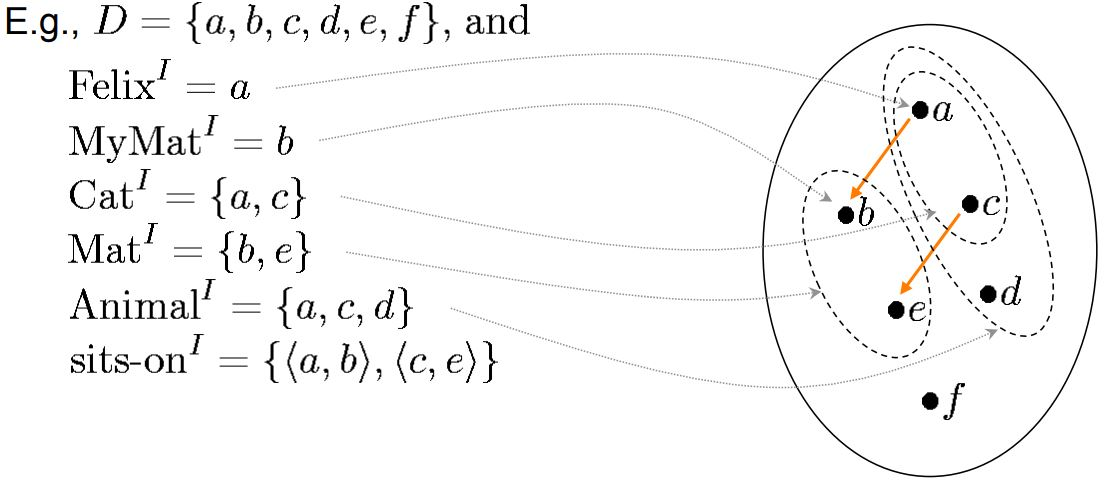
\includegraphics[width=\textwidth]{FOL.JPG}
  \caption{First-order Logic}
  \label{fig:FOL}
\end{figure}

Table \ref{table:FOL_truth_evaluation} shows some truth value evaluation examples in the above given model $M = <D, .^{I}>$, see figure \ref{fig:FOL} for model definition.

\begin{longtable}[h]{ p{100mm} p{30mm} }
\caption{FOL Truth value evaluation}
\label{table:FOL_truth_evaluation}\\
\hline
Statement & Evaluation\\
\hline
$\exists x.Cat(x)$ & true\\
$\forall x.Cat(x)$ & false\\
$\exists x.Cat(x) \land Mat(x)$ & false\\
$\forall x.Cat(x) \rightarrow Animal(x)$ & true\\
$\forall x.Cat(x) \rightarrow (\exists y.Mat(y) \land sits-on(x,y))$ & true\\
\hline
\end{longtable}

\subsubsection{Satisfiability and Decidability}
\label{sec:satisfiability_decidability}

Given a model M and a formula F, M is a model of F (written $M \models F$) iff F evaluates to true in M.
See examples below.

$M \models \exists x.Cat(x)$

$M \not\models \forall x.Cat(x)$

$M \not\models \exists x.Cat(x) \land Mat(x)$

$M \models \forall x.Cat(x) \rightarrow Animal(x)$

$M \models \forall x.Cat(x) \rightarrow (\exists y.Mat(y) \land sits-on(x,y))$

A formula F is \textbf{satisfiable} iff there exists a model M s.t. $M \models F$.

A formula F \textbf{entails} another formula G (written $F \models G$) iff every model of F 
is also a model of G (i.e., $M \models F$ implies $M \models G$). 

Satisfiable examples:

$Cat(Felix) \models \exists x.Cat(x)$

$(\forall x.Cat(x) \rightarrow Animal(x)) \land Cat(Felix) \models Animal(Felix)$

$(\forall x.Cat(x) \rightarrow Animal(x)) \land \neg Animal(Felix) \models \neg Cat(Felix)$

Not satisfiable:

$Cat(Felix) \models \forall x.Cat(x)$

$sits-on(Felix, Mat1) \land sits-on(Tiddles, Mat2) \models \neg sits-on(Felix, Mat2)$

$sits-on(Felix, Mat1) \land sits-on(Tiddles, Mat1) \models \exists^{\geq 2} x.sits-on(x, Mat1)$

Satisfiability in the first-order logic is undecidable, i.e. no algorithm can decide correctly whether a given first-order formula is true or not. However, for any single statement $\varphi$ it is easy to come up with an algorithm that decides $\varphi$ correctly (just hard-code the answer). 
You can encode the statement \textbf{"the Turing machine T halts on empty input"} in first-order logic, this statement is already undecidable, that is, no algorithm can correctly decide whether such a formula is true or not, 
see section \ref{sec:halting_problem} about why. 
Other logics (propositional logic, DL) is decidable because they don't have the power to encode such statement \cite{30672}.

Example decidable fragments: FOL with Counting quantifiers ($\exists^{\geq n}, \exists^{\leq n}$)

$\exists^{\geq 3}x.Cat(x)$ equivalent to

$\exists x,y,z.Cat(x) \land Cat(y) \land Cat(z) \land x \neq y \land x \neq z \land y \neq z $

$\exists^{\leq 2}x.Cat(x)$ equivalent to

$\forall x,y,z.Cat(x) \land Cat(y) \land Cat(z) \rightarrow x=y \lor x=z \lor y=z $

\subsubsection{Halting Problem}
\label{sec:halting_problem}
In computability theory, the halting problem is the problem of determining, from a description of an arbitrary computer program and an input, whether the program will finish running or continue to run forever.

Alan Turing proved in 1936 that a general algorithm to solve the halting problem for all possible program-input pairs cannot exist. A key part of the proof was a mathematical definition of a computer and program, which became known as a Turing machine; the halting problem is undecidable over Turing machines. It is one of the first examples of a decision problem \cite{halting_problem}.

Proof by contradiction:
Suppose that there exists a total computable function \textbf{halts(g)} that returns true if the subroutine g halts (when run with no inputs) and returns false otherwise. Now consider the following subroutine:
\begin{lstlisting}
def g():
    if halts(g):
        loop_forever()
\end{lstlisting}
\textbf{halts(g)} must either return true or false, because halts was assumed to be total. 
If \textbf{halts(g)} returns true, then g will call \textbf{loop\textunderscore forever} 
and never halt, which is a contradiction. 
If \textbf{halts(g)} returns false, then g will halt, 
because it will not call \textbf{loop\textunderscore forever}; this is also a contradiction. 
Overall, \textbf{halts(g)} can not return a truth value that is consistent with whether g halts. 
Therefore, the initial assumption that halts is a total computable function must be false.

\subsection{Knowledge Base}
\label{sec:KB}

A knowledge base (KB) \cite{knowledge_base} is a technology used to store complex structured and unstructured information used by a computer system. A knowledge-based system consists of a knowledge-base that represents facts about the world and an inference engine \cite{jena} that can reason about those facts and use rules and other forms of logic to deduce new facts or highlight inconsistencies.

The term "knowledge-base" was coined to distinguish this form of knowledge store from the more common and widely used term database. At the time (the 1970s) virtually all large Management Information Systems stored their data in some type of hierarchical or relational database. At this point in the history of Information Technology the distinction between a database and a knowledge base was clear and unambiguous. A database had ACID transaction properties: Atomicity, Consistency, Isolation, and Durability. Early expert systems had little need for the complexity that comes with requiring transactional properties on data. 

The volume requirements were also different for a knowledge-base compared to a conventional database. The knowledge-base needed to know facts about the world. For example, to represent the statement that "All humans are mortal". A database typically could not represent this general knowledge but instead would need to store information about thousands of tables that represented information about specific humans. Representing that all humans are mortal and being able to reason about any given human that they are mortal is the work of a knowledge-base. Representing that George, Mary, Sam, Jenna, Mike,... and hundreds of thousands of other customers are all humans with specific ages, sex, address, etc. is the work for a database.

The next evolution for the term knowledge-base was the Internet. With the rise of the Internet, documents, hypertext, and multimedia support were now critical for any corporate database. It was no longer enough to support large tables of data or relatively small objects that lived primarily in computer memory. 

Knowledge Base Consistency Checking:
Given knowledge base K as input, a decision procedure for knowledge base consistency returns “K is consistent” if there is an interpretation I such that $I \models K$, otherwise it returns “K is inconsistent.” \cite{KnowledgeBaseConsistency}, see section \ref{sec:satisfiability_decidability} for more definitions. 

Some example knowledge base datasets:

\begin{enumerate}
    % 1
    \item 
    DBpedia – a dataset containing extracted data from Wikipedia; it contains about 3.4 million concepts described by 1 billion triples, including abstracts in 11 different languages.
    % 2
    \item
    FOAF \cite{FOAF} – a dataset describing persons, their properties and relationships.
    % 3
    \item
    GeoNames provides RDF descriptions of more than 7,500,000 geographical features worldwide.
     % 4
    \item
    Wikidata – a collaboratively-created linked dataset that acts as central storage for the structured data of its Wikimedia Foundation sister projects.In 2014, Freebase \cite{Freebase} merged into Wikidata, Google's Knowledge Graph was powered in part by Freebase.
\end{enumerate}
